% ===============================================================
%
%  Template for creating scribe notes for CS:3330, Algorithms.             I am using this template to get my homework PDF's set up as well
%
%  Fill in your name, lecture date, and body of scribe notes
%  as indicated below.
%
% ===============================================================

\documentclass[11pt]{article}

\usepackage{graphicx}
\usepackage{amssymb, amsthm}
\usepackage{pgfplots}
\usepackage{tikz}
\usetikzlibrary{datavisualization}
\usetikzlibrary{datavisualization.formats.functions}



\setlength{\topmargin}{0pt}
\setlength{\textheight}{9in}
\setlength{\headheight}{0pt}
\setlength{\headsep}{0pt}
\setlength{\oddsidemargin}{0.25in}
\setlength{\textwidth}{6in}

\pagestyle{plain}

\begin{document}

\thispagestyle{empty}

\begin{center}
\bf\large CS:3330, Algorithms
\end{center}

\begin{center}
\bf\large HW03 Algorithm Efficiency Problems    %Fill in Name of Homework here
\end{center}

\noindent
Logan Zweifel     % FILL IN YOUR NAME HERE
\hfill
September 5, 2021           % FILL IN HW DATE HERE

\noindent
\rule{\textwidth}{1pt}

\medskip

%%%%%%%%%%%%%%%%%%%%%%%%%%%%%%%%%%%%%%%%%%%%%%%%%%%%%%%%%%%%%%%%
% BODY OF HOMEWORK NOTES GOES HERE
%%%%%%%%%%%%%%%%%%%%%%%%%%%%%%%%%%%%%%%%%%%%%%%%%%%%%%%%%%%%%%%%

%%%%%%%%%%% 1
\section{$f(n)$ and $f(8n)$}
For each of the following functions, indicate how much the function's value will change if its argument is increased eightfold. Use either (i) the difference between,
 or (ii) the ratio of $f(8n)$ and $f(n)$, whichever is more convenient for getting a compact answer. Note that none of the answers depend on n.

%a
\subsection*{a) $f(n) = lg (n)$}
First, it is important to note that $lg (n)$ is shorthand for $log_2 (n)$. Next, $f(8n)$ is represented by the expression $lg (8n)$.
Using the logarithm product rule:

\begin{verbatim}
     log(x*y) = log(x) + log(y)
\end{verbatim}

\noindent $f(8n)$ can be simplified.

\begin{eqnarray*}
f(8n) &=& lg(8n) \\
&=& lg(8) + lg(n)\\
&=& lg(n) + 3
\end{eqnarray*}

Therefore, for $f(n) = lg(n)$, when the argument is increased eightfold, the value of $f(8n)$ will be 3 greater than the value of $f(n)$. A graphic representation of this is below and is included for all problems (a-e).

\begin{center}
\begin{tikzpicture}[scale=0.75]
\datavisualization    [school book axes,
			visualize as smooth line/.list={n,8n},
			y axis={label={$f(n)$}, length = 5cm},
			x axis={label={$n$}, length= 5cm, ticks=few},
                    		style sheet=strong colors,
                    		n={label in legend={text=$f(n)$}},
                    		8n={label in legend={text=$f(8n)$}},
                    		data/format=function
                    		]
data [set=n] {
  var x : interval [0.01:10];
  func y = log2(\value x);
}
data [set=8n] {
  var x : interval [0.01:10];
  func y = log2(\value x*8);
};
\end{tikzpicture}
\end{center}

%b
\subsection*{b) $f(n) = \sqrt[3]{n}$}
For $f(n) = \sqrt[3]{n}$, $f(8n)$ is represented by the expression $\sqrt[3]{8n}$. Using the multiplication rule for roots and radicals: 
$\sqrt{xn} = \sqrt{x} * \sqrt{n}$ , this expression can be simplified.

\begin{eqnarray*}
f(8n) &=& \sqrt[3]{8n}\\
&=& \sqrt[3]{8} * \sqrt[3]{n}\\
&=& 2 * \sqrt[3]{n}
\end{eqnarray*}

Therefore, the value of $f(8n)$ wll be twice than that of the value of $f(n)$.

\begin{center}
\begin{tikzpicture}[scale=0.75]
\datavisualization    [school book axes,
			visualize as smooth line/.list={n,8n},
			y axis={label={$f(n)$}, length = 5cm, ticks=few},
			x axis={label={$n$}, length= 5cm, ticks=few},
                    		style sheet=strong colors,
                    		n={label in legend={text=$f(n)$}},
                    		8n={label in legend={text=$f(8n)$}},
                    		data/format=function
                    		]
data [set=n] {
  var x : interval [0:10];
  func y = \value x^(1/3);
}
data [set=8n] {
  var x : interval [0:10];
  func y = (\value x*8)^(1/3);
};
\end{tikzpicture}
\end{center}

%c
\subsection*{c) $f(n) = n$}
For $f(n) = n$, $f(8n)$ is represented by the expression $8n$. Therefore, for all values of n except 0, the value of $f(8n)$ will be 8 times more 
positive or negative (depending on the sign of the argument) than the value of $f(n)$. When n is 0, both have a value of 0.

\begin{center}
\begin{tikzpicture}[scale=0.75]
\datavisualization    [school book axes,
			visualize as smooth line/.list={n,8n},
			y axis={label={$f(n)$}, length = 5cm, ticks=few},
			x axis={label={$n$}, length= 5cm, ticks=few},
                    		style sheet=strong colors,
                    		n={label in legend={text=$f(n)$}},
                    		8n={label in legend={text=$f(8n)$}},
                    		data/format=function
                    		]
data [set=n] {
  var x : interval [-10:10];
  func y = \value x;
}
data [set=8n] {
  var x : interval [-10:10];
  func y = \value x*8;
};
\end{tikzpicture}
\end{center}


%d
\subsection*{d) $f(n) = n^2$}
For $f(n) = n^2$, $f(8n)$ is represented by the expression $64n^2$. Therefore, for all values of n except 0, the value of $f(8n)$ will be 64 times more 
than the value of $f(n)$. When n is 0, both have a value of 0. Because of the large difference between these two functions, you can't start to see $f(n)$ come off of the x-axis until the edge of the graph.


\begin{center}
\begin{tikzpicture}[scale=0.75]
\datavisualization    [school book axes,
			visualize as smooth line/.list={n,8n},
			y axis={label={$f(n)$}, length = 5cm, ticks=few},
			x axis={label={$n$}, length= 5cm, ticks=few},
                    		style sheet=strong colors,
                    		n={label in legend={text=$f(n)$}},
                    		8n={label in legend={text=$f(8n)$}},
                    		data/format=function
                    		]
data [set=n] {
  var x : interval [-10:10];
  func y = \value x*\value x;
}
data [set=8n] {
  var x : interval [-10:10];
  func y = \value x*\value x*64;
};
\end{tikzpicture}
\end{center}

%e
\subsection*{e) $f(n) = n^3$}
For $f(n) = n^3$, $f(8n)$ is represented by the expression $512n^3$. Therefore, for all values of n except 0, the value of $f(8n)$ will be 512 times more 
positive or negative (depending on the sign of the argument) than the value of $f(n)$. When n is 0, both have a value of 0. In the graph below, the differences between the two functions is so great that you can't see the black line of $f(n)$ very well as it is right on the x-axis.

\begin{center}
\begin{tikzpicture}[scale=0.75]
\datavisualization    [school book axes,
			visualize as smooth line/.list={n,8n},
			y axis={label={$f(n)$}, length = 5cm, ticks=few},
			x axis={label={$n$}, length= 5cm, ticks=few},
                    		style sheet=strong colors,
                    		n={label in legend={text=$f(n)$}},
                    		8n={label in legend={text=$f(8n)$}},
                    		data/format=function
                    		]
data [set=n] {
  var x : interval [-2:2];
  func y = \value x*\value x*\value x;
}
data [set=8n] {
  var x : interval [-2:2];
  func y = \value x*\value x*\value x*512;
};
\end{tikzpicture}
\end{center}

%%%%%%%%%%%%%%%%%%%2
\section{Sequential Search Efficiency}
Consider a variation of sequential search that scans a list to return the number of occurrences of a given search key in the list. Does its efficiency differ 
from the efficiency of classic sequential search? Your answer should include three parts, one each for Best Case, Average Case, and Worst Case time 
efficiencies. Explain your answers.

\bigskip 

\bigskip

The efficiency of this modified sequential search algorithm will differ from the original. The modified algorithm must traverse and compare every single item in the list, and therefore it has a every-case time complexity of $T(n)= n$ rather than a different time complexity for best, average, and worst case. Overall, the modified algorithm will run slower than the original for all cases except for the worst case of the classic sequential search.

%BC
\subsection*{Best-Case Time Complexity}
Since the modified sequential search algorithm has an every-case time complexity, it's best-case time complexity would be the exact same as the every-case time complexity ($T(n)=B(n)=n$). Comparing this to the best-case for the original sequential search algorithm with a $B(n)=1$, and there is an obvious massive difference between the two. As the input size gets larger the original best-case will only continue to be more efficient than that of the modified because it is has more comparisons to do as a result of a bigger array to traverse.


%AC
\subsection*{Average-Case Time Complexity}
Since the modified sequential search algorithm has an every-case time complexity, it's average-case time complexity would be the exact same as the every-case time complexity ($T(n)=A(n)=n$). The original sequential search has average-time complexities for two different cases. The first is when it is known that x is in the array where $A(n)= (n+1)/2$. The second case is when it is not known that x is in the array where $A(n)=n(1-(p/2))+(p/2)$. For both these cases, it can be expected that classical sequential search will go on average about halfway through the array which would generally then be twice as efficient as the modified sequential search which has the time complexity of $n$.


%WC
\subsection*{Worst-Case Time Complexity}
Since the modified sequential search algorithm has an every-case time complexity, it's worst-case time complexity would be the exact same as the every-case time complexity ($T(n)=W(n)=n$). In this case, the worst-case for the original sequential search is the same as the worst-case for the modified. For both these algorithms, it means that they traversed through the entire list and compared every item to the key.



%%%%%%%%%%%%%%%%%%%%%%3
\section{Constant-time Operation}
Desribe how to implement a constant-time operation on an unsorted list of size n that deletes the ith element ($0 <= i < n$). Remember, the running time of this operation must be constant; in other words the running time must not depend on the number of items in the list.

\bigskip 

\bigskip

To create a constant-time operation to fulfil this goal you simply need to utilize some built in methods for python lists. Specifically the use of the pop method will remove the element at the specified index of the list, S.remove(i), and then you can replace that index with the last element in the list and decrease the length of the list by one. Both the pop, replacement, and shortening of the index and list as a whole operate independent of any input size n given that the assumption ($0 <= i < n$) is true.

%%%%%%%%%%%%4
\section{Algorithm A and B}
Algorithm A performs $966n^2$ basic operations, and algorithm B performs $24n^3$ basic operations. For what value of $n$ does algorithm A start to show its better performance?

\bigskip 

\bigskip

By setting the number of basic operations of the two algorithms equal to each other, you can find the value of n for which they perform the same.

\begin{eqnarray*}
966n^2 &=& 24n^3 \\
40.25 &=& n
\end{eqnarray*}

Specifcally, at $n=40.25$, Algorithm A starts performing better than algorithm B. However, if only going by whole numbers, Algorithm A would start to perform better at $n=41$. This relates to Big O notation and the growth of functions. Because both algorithms are represented by polynomials, no matter how long it takes, the algorithm with the smaller degree will perform better as it goes towards infinity.


%%%%%%%%%%%%%%%%5
\section{Algorithm 1 and 2 justification for use}
There are two algorithms called Algo1 and Algo2. For an input size of $n$, Algo 1 runs in $n^3$ microseconds and Algo2 runs in $200nlogn$ microseconds. Algo1 can be implemented using 6 hours of programmer time and 7 minutes of CPU time. On the other hand, Algo2 requires 22 hours of programmer time and 12 minutes of CPU time to implement. If programmers are paid $25 per hour and CPU time costs $60 per minute, how many times must a problem of size $n = 600$ be solved using Algo2 to justify its development cost? 

\bigskip 

\bigskip

The first step is to find the start up costs and cost per iteration of the problem for both Algorithms. For algorithm 1, the total implementation cost is \$570, as a sum of \$120 from 6 hours of programming time at \$25 per hour and \$420 from 7 minutes of CPU time at \$60 per minute. The cost per iteration is gained by the following and the final equation incorporates the cost of implementation in at the end:

\begin{eqnarray*}
(600^3*10^{-6}*(1/60)*(60/1))x &=& (600^3*10^{-6})x \\
&=& (216000000*10^{-6})x \\
&=& (216)x \\
&=& 570 + 216x
\end{eqnarray*}

In these equations in the first line, the $(1/60)$ and $(60/1)$ represent the conversion from seconds to minutes and the cost of CPU time per minute respectively. In the case of this problem, these two cancel each other out. For algorithm 2, the total implementation cost is \$1,270, as a sum of \$550 from 22 hours programming time at \$25 per hour and \$720 from 12 minutes CPU time at \$60 per minute. The cost per iteration is gained the same way as was done for algorithm 1 and the total cost of implementation is agian not added until the final equation.

\begin{eqnarray*}
(200*600*log600*10^{-6}* (1/60)*(60/1)x &=& (200*600*log600*10^{-6})x \\
&=& (333378.15*10^{-6})x\\
&=& (0.33337815)x\\
&=& 1270 + 0.33337815x
\end{eqnarray*}

Now, setting these equations equal to each other and solving for x will give the result of how many times algo2 to must solve a problem of size $n=600$ to justify its development cost.

\begin{eqnarray*}
570 + 216x &=& 1270 + 0.33337815x \\
216x - 0.33337815x &=& 1270-570\\
215.6666219x &=& 700 \\
x &=& 3.24575
\end{eqnarray*}

The number of times that algo2 must run the problem with a size of 600 is 3.24575 times. The number of times it needs to run itself to prove its worth despite having a much more expensive total implementation cost is because how much more effecient the growth of a function of $nlogn$ is than a polynomial function, $n^3$. If the degree of polynomial were lower the number of problems that would need to be run to prove the worth of algorithm two would be in the hundreds rather than under 10. 

%%%%%%%%%%%%%%%%%%%%%%%%%%%%%%%%%%%%%%%%%%%%%%%%%%%%%%%%%%%%%%%%

\end{document}






























